We can visualize a function, \(f,\) by plotting many (maybe 10 or maybe 100) of the ordered pairs of the form \((x,f(x))\) and then connecting them with straight lines. The more points we plot the more accurate this will be. Below, we have a demonstration of this effect with the function \(f(x) = \frac{1}{x^2+1}\). On the left, the computer plotted this function with \(50\) points of the form \((x,f(x)).\) On the right, the computer used only \(5\) such points. In both drawings, the point \((1,0.5)\) is plotted. Notice that it visibly does not lie on the line meant to represent the function despite the fact that \(f(1)=0.5.\) 

\begin{image}
\begin{tikzpicture}
  \begin{axis}[
  xmin=-0.5,
  xmax=2.5,
  ymin=-.5,
  ymax=1.2,
  axis lines=center,
  xlabel=$x$,
  ylabel=$y$,
  every axis y label/.style=
    {at=(current axis.above origin),anchor=south},
  every axis x label/.style=
    {at=(current axis.right of origin),anchor=west},
  ]
\addplot [very thick, blue, smooth, samples=50] {1/(x^2+1)};
\addplot[dashed, domain = 0:1]{1/2};
\addplot[dashed] coordinates {(1,0) (1,1/2)};
\addplot[mark=*] coordinates {(1,1/2)};
\end{axis}
\end{tikzpicture}

\begin{tikzpicture}
  \begin{axis}[
  xmin=-0.6,
  xmax=2.6,
  ymin=-.5,
  ymax=1.2,
  axis lines=center,
  xlabel=$x$,
  ylabel=$y$,
  every axis y label/.style=
    {at=(current axis.above origin),anchor=south},
  every axis x label/.style=
    {at=(current axis.right of origin),anchor=west},
  ]
\addplot [very thick, blue, samples=7] {1/(x^2+1)};
\addplot[dashed, domain = 0:1]{1/2};
\addplot[dashed] coordinates {(1,0) (1,1/2)};
\addplot[mark=*] coordinates {(1,1/2)};
\end{axis}
\end{tikzpicture}
\end{image}

Recall the definition of a function.

\begin{definition}
    A function -- which we will call \(f\) -- from a set \(X\) to a set \(Y\) is a rule that assigns to each \(x\) in \(X\) exactly one element of \(Y.\) The element of \(Y\) which is assigned to \(x\) is denoted \(f\left(x\right).\) The set \(X\) is called the domain and the subset of \(Y\) consisting of all \(f\left(x\right)\) is called the range of \(f.\)
\end{definition}

In terms of the graph of a function, the ``...exactly one element of \(Y\)'' part of this definition can be interpreted in terms of vertical lines.

\begin{theorem}[The vertical line test] A subset of \(xy\)-plane is a function if every vertical line meets the subset at most one time. Moreover, if the vertical line \(x=a\) passes through this subset then \(a\) is in the domain of the function. 
\end{theorem}

In the image below, a vertical line passes through twice. Hence, this line cannot represent a function of the form \((x,f(x)).\)

\begin{image}
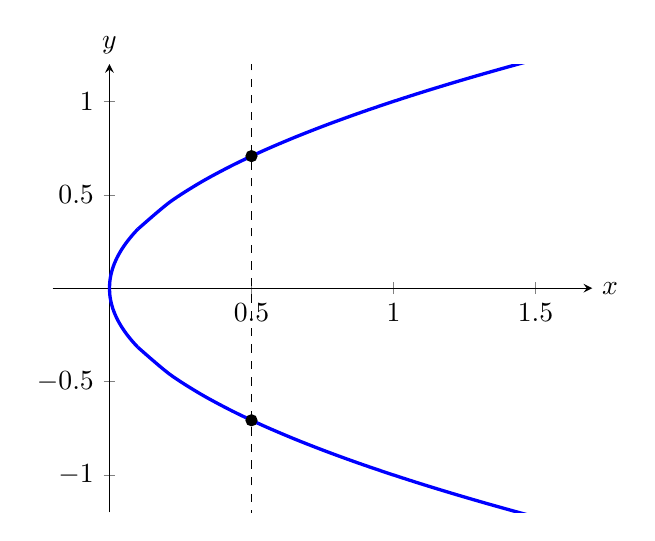
\begin{tikzpicture}
  \begin{axis}[
  xmin=-0.2,
  xmax=1.7,
  ymin=-1.2,
  ymax=1.2,
  axis lines=center,
  xlabel=$x$,
  ylabel=$y$,
  every axis y label/.style=
    {at=(current axis.above origin),anchor=south},
  every axis x label/.style=
    {at=(current axis.right of origin),anchor=west},
  ]
\addplot [very thick, blue, smooth, samples=100, domain = 0:0.1] { sqrt(x) };
\addplot [very thick, blue, smooth, samples=20, domain = 0.1:2.2] { sqrt(x) };
\addplot [very thick, blue, smooth, samples=100, domain = 0:0.1] { -sqrt(x) };
\addplot [very thick, blue, smooth, samples=20, domain = 0.1:2.2] { -sqrt(x) };
\addplot[dashed] coordinates {(.5,-1.5) (0.5,1.5)};
\addplot[mark=*] coordinates {(1/2,0.7071)};
\addplot[mark=*] coordinates {(1/2,-0.7071)};
\end{axis}
\end{tikzpicture}
\end{image}